% !TeX root = ../thuthesis-example.tex

\chapter{实验设计与仿真验证}
\label{sec:experiment}

\section{实验方法总览}
本节先对多源数据进行统一字段映射、样本过滤与张量化缓存构建，再在统一超参数口径下训练MLP基准推荐模型并以验证集指标监控训练过程，随后计算 SIF、Influence Function、TracIn 与 DVF 的样本级分数，并在统一 benchmark 协议下通过 deletion/insertion/NDCG 曲线及其面积指标、随机基线校正与多种子统计检验联合评估方法效果，从而在“可比性、可解释性与可复核性”三个维度形成闭环。

\section{数据来源}
本文实验数据采用三类公开推荐基准数据：MovieLens1M、Yahoo!Music 子集与 Pinterest 子集。为保证跨方法比较的公平性，本文在同一数据来源下执行统一字段映射与预处理。

\section{阶段一：统一数据准备与缓存}
在数据准备阶段，首先将不同公开推荐数据的原始交互字段统一映射为 user-item-label 三元表示，并通过最小交互阈值过滤稀疏噪声样本；随后构建训练/验证划分及样本标识，生成统一的张量化缓存（含稀疏特征、稠密特征、标签与样本ID），用于后续模型共享输入接口。该阶段的设计目标是避免数据格式差异对归因结论产生干扰。

\section{阶段二：MLP基准推荐模型训练}
在统一输入表示上，训练 MLP 基准推荐模型，并采用一致的训练设置（学习率、批大小与验证划分比例）。训练过程中按 epoch 记录验证损失、准确率与AUC，确保后续归因比较在统一评测口径下进行。

\section{阶段三：SIF与阶段DVF估值}
在完成基准训练后，基于保存的模型状态计算样本级价值分数。具体地，SIF以样本梯度与验证梯度内积作为一次性代理分数；阶段DVF则在多个训练阶段快照上累计样本影响，并输出总价值与分阶段价值（stage1、stage2），用于刻画数据价值在训练过程中的时序变化。该阶段输出样本级估值表及高/低价值样本列表，支持后续解释分析。

\section{阶段四：小样本归因对比验证}
为验证估值指标的有效性，进一步在小样本设置下进行归因对比实验：先从训练与验证集合中分别抽取固定规模子集，并在该子集上按统一效用函数生成各方法样本排序；再基于排序计算 deletion 曲线、insertion 曲线与 NDCG@Ke 曲线，并积分得到 deletion\_auc、insertion\_auc 与 ndcg\_ke\_auc，同时报告 pos@10 与方法耗时。为控制排序随机性的影响，实验对随机排序进行重复采样并构建随机参考值，最终同时报告原始指标与相对随机基线增益指标。

\section{方法实现与复现说明}
上述四阶段流程采用模块化实现：共享函数负责数据解析、模型构建与估值算子，流程层负责顺序执行与中间结果落盘。该实现方式使实验步骤、关键超参数与输出产物具备可追踪性，便于复现实验与开展增量对比。

\section{验证口径}
本文在实验验证中采用以下的统一设置：
\begin{itemize}
    \item \textbf{数据划分与子样本预算：}按随机种子进行 train/val 划分（val\_ratio=$0.2$，batch\_size=$256$），并在评测阶段固定子样本规模（$n\_{train}=96$、$n\_{val}=256$）以控制计算预算。
    \item \textbf{效用函数构造：}在训练子样本子集上执行短程重训练（epochs\_in\_utility=$14$，lr=$1\\times10^{-3}$），以验证集 AUC 作为效用值，并通过重复训练取平均降低估计方差。
    \item \textbf{曲线与面积指标：}在 deletion\_fracs 与 insertion\_fracs（$\{0.05,0.1,0.2,0.3,0.4\}$）上计算 deletion/insertion 曲线及 AUC，在 ndcg\_ke（$\{5,10,20\}$）上计算 NDCG 曲线并积分得到 ndcg\_ke\_auc，同时报告 pos@10。
    \item \textbf{随机基线校正：}随机排序重复采样（random\_repeats=$7$），并以中位数聚合得到随机参考值；主结果同时报告原始指标与减随机基线增益指标。
    \item \textbf{多随机种子统计：}采用 $5$ 个随机种子重复实验，报告 mean$\pm$std，并对 SIF 与 Influence Function、DVF、TracIn 的差异使用 Wilcoxon signed-rank 检验与 Cliff's $\delta$ 效应量检验。
\end{itemize}

\section{结果边界与后续工作说明}
为避免读者对当前结果的解释范围产生误解，本文声明：主文报告已完成实验部分对应的证据范围；对于尚在推进中的部分，我们在此仅给出后续验证计划，不将其提前写入正文的结论。
\begin{itemize}
    \item \textbf{解释边界：}本文将结果定位为趋势性证据（trend-level evidence）；对未达到校正后显著性门槛的比较，不作确定性优越判断。
    \item \textbf{评测一致性：}后续补充实验将保持同一评测协议（seed 方案、随机基线聚合、Wilcoxon 与 Holm 校正、Cliff's $\delta$），以保证不同阶段结果可比。
    \item \textbf{可追踪披露：}新增结果将以“时间戳+配置快照+输出文件清单”的方式给出，便于读者核对差异来源。
    \item \textbf{完整呈现：}后续报告将同时呈现显著与不显著结果，尽量降低选择性展示带来的偏差。
\end{itemize}

\section{主结果}
本节给出到本文截稿日为止的有效实测结果。表 \ref{tab:main_result} 中指标来自同一评测口径下的 5 个随机种子统计，数值以 mean$\pm$std 形式报告；统计列基于 Wilcoxon 检验与 Holm 校正结果。

\begin{table}[htbp]
\centering
\caption{主结果（一）：归因质量与运行耗时（MLP，5 seeds，mean$\pm$std）}
\label{tab:main_result}
\small
\begin{tabular}{@{}lcccc@{}}
\toprule
方法 & Deletion-AUC$\uparrow$ & Insertion-AUC$\uparrow$ & NDCG@Ke-AUC$\uparrow$ & 用时(s)$\downarrow$ \\\midrule
SIF             & $0.0669\pm0.0248$ & $0.1419\pm0.0334$ & $33.75\pm4.42$ & $1.1128\pm0.1776$ \\
SIF+            & $0.0683\pm0.0209$ & $0.1513\pm0.0216$ & $35.43\pm2.80$ & $1.3953\pm0.1099$ \\
Infl.\ Func.    & $-0.0091\pm0.0066$ & $0.0689\pm0.0124$ & $27.20\pm7.59$ & $1.5431\pm0.1459$ \\
DVF             & $0.0691\pm0.0261$ & $0.1402\pm0.0385$ & $33.85\pm3.78$ & $27.8705\pm0.5167$ \\
TracIn          & $0.0689\pm0.0257$ & $0.1408\pm0.0394$ & $33.89\pm3.68$ & $27.8701\pm0.5167$ \\\bottomrule
\end{tabular}
\end{table}

\begin{table}[htbp]
\centering
\caption{主结果（二）：Wilcoxon 检验与 Holm 校正结果}
\label{tab:main_stat}
\small
\begin{tabular}{@{}lcc@{}}
\toprule
方法 & vs.\ SIF+（Holm $p$） & vs.\ SIF（Holm $p$） \\\midrule
SIF             & 未显著（$p=1.000$）     & 参考方法 \\
SIF+            & 参考方法                & 未显著（$p=1.000$） \\
Infl.\ Func.    & 未显著（$p\geq0.625$） & 未显著（$p\geq0.625$） \\
DVF             & 未显著（$p=1.000$）     & 未显著（$p=1.000$） \\
TracIn          & 未显著（$p=1.000$）     & 未显著（$p=1.000$） \\\bottomrule
\end{tabular}
\end{table}

\begin{figure}[H]
\centering
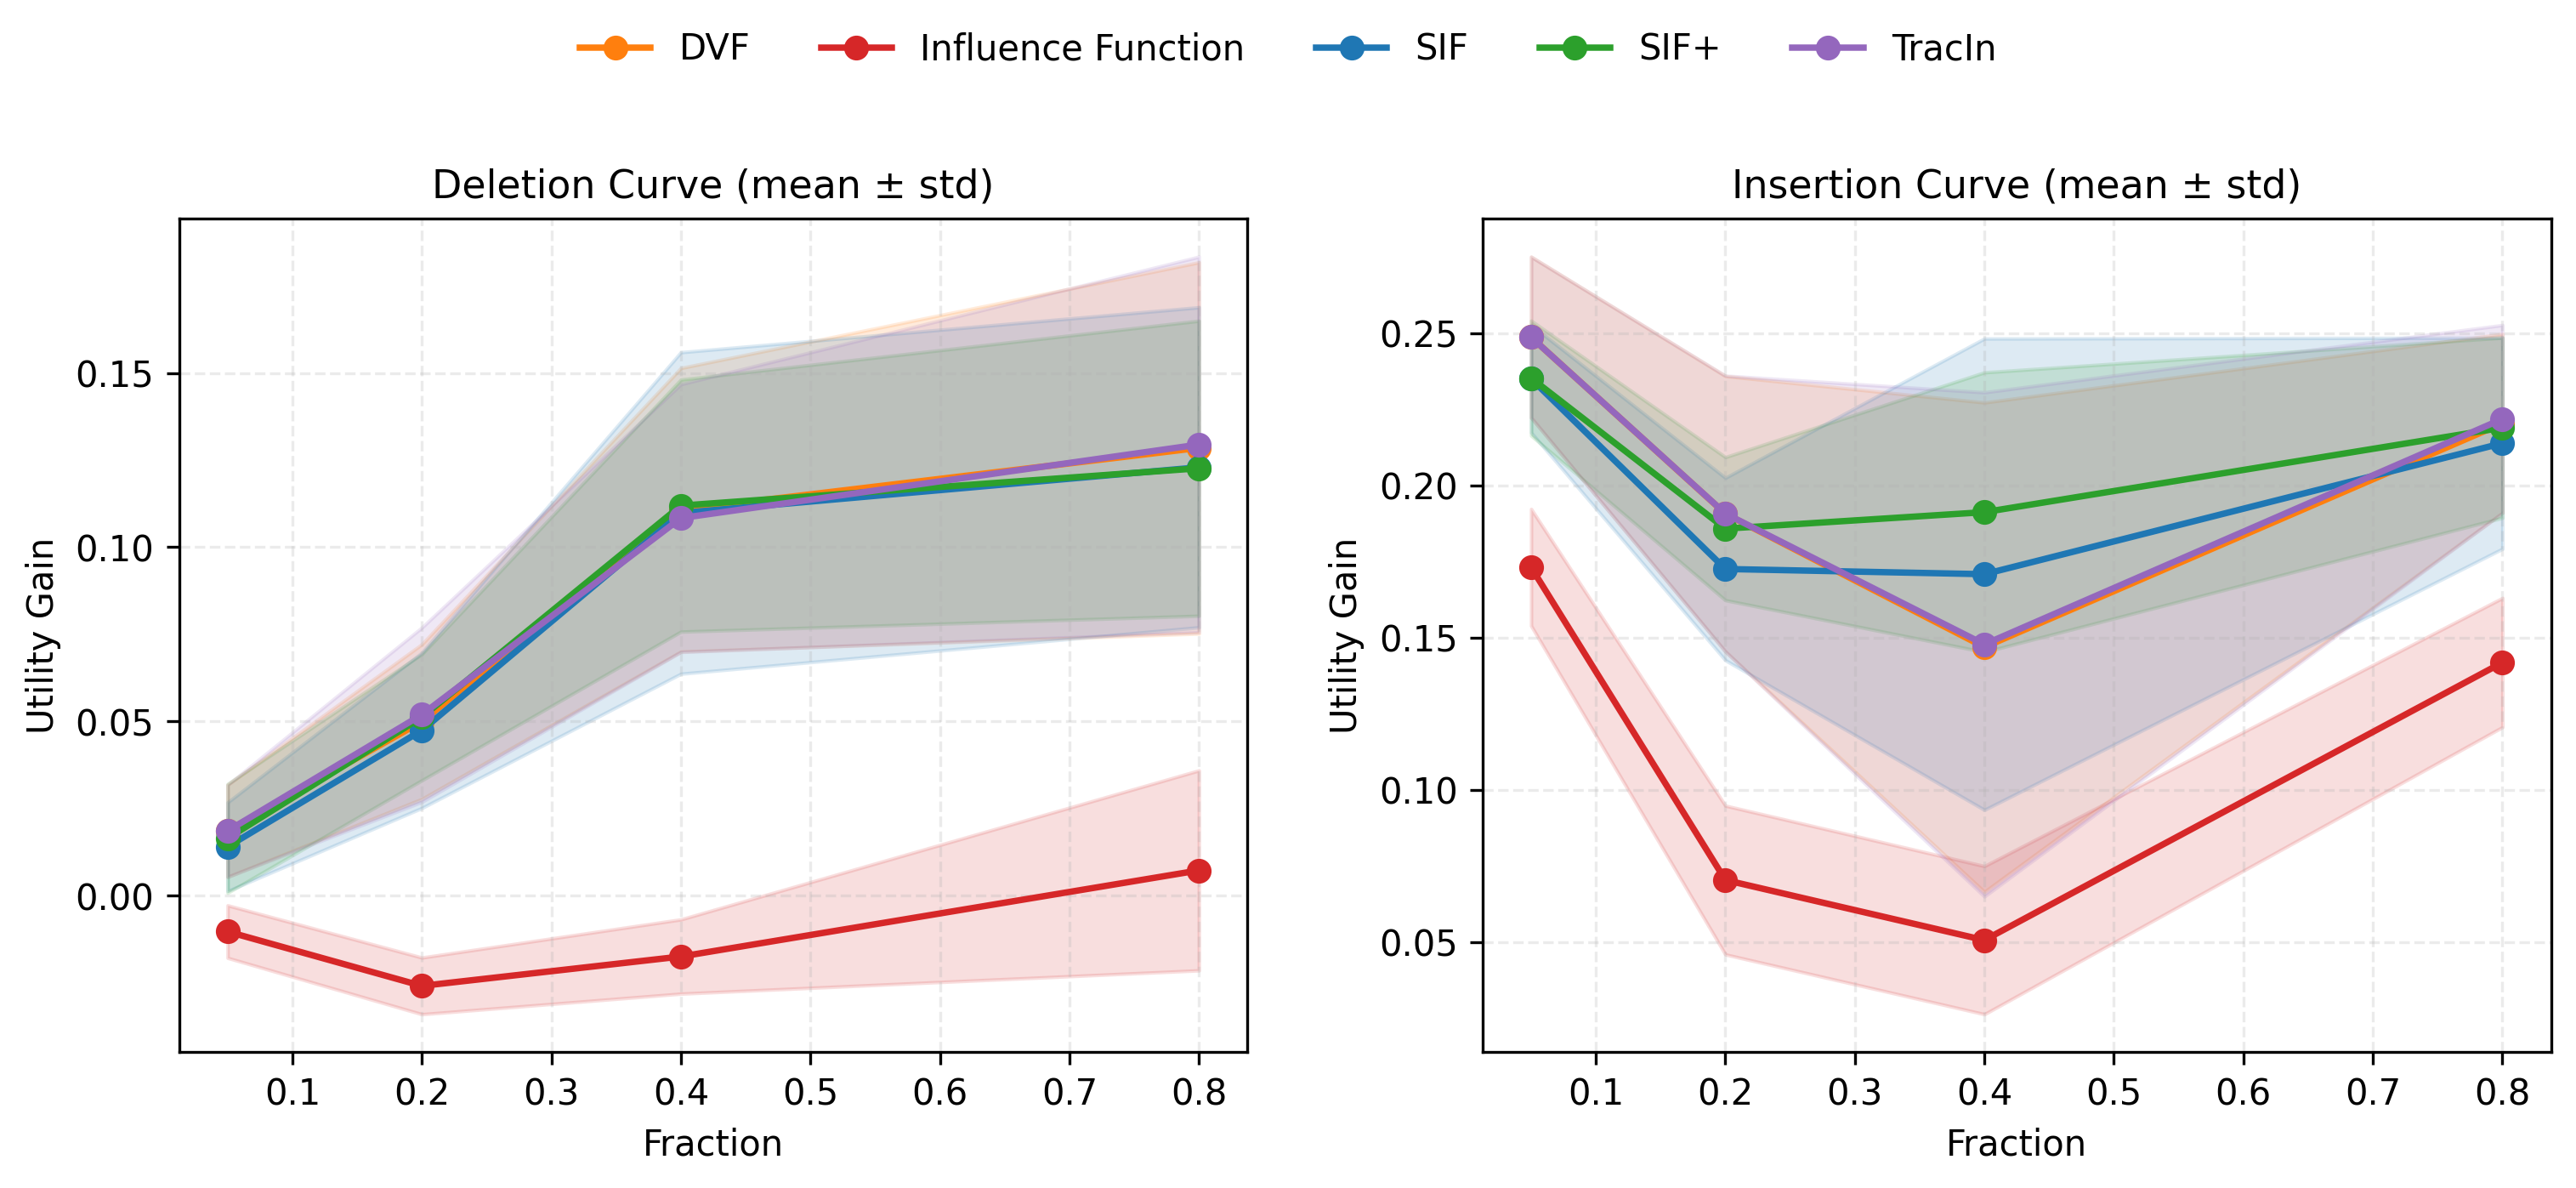
\includegraphics[width=\textwidth]{figures/del&ins_auc.png}
\caption{删除与插入AUC曲线}
\label{fig:del_ins_auc}
\end{figure}

